\documentclass[tikz,border=11pt]{standalone}
\usepackage{lmodern}
\usetikzlibrary{shadings,calc}
% The graph K_3^# of the paper: each edge of the triangle xyz becomes a path of length four and each
% vertex gets a pendant vertex. Edges are ordered (x,y), (y,z), (x,z). Shaded vertices form the set
% J(I) for I = {x}, a largest 2-independent set and a largest minimal 2-star-forming set (10 vertices).
\begin{document}
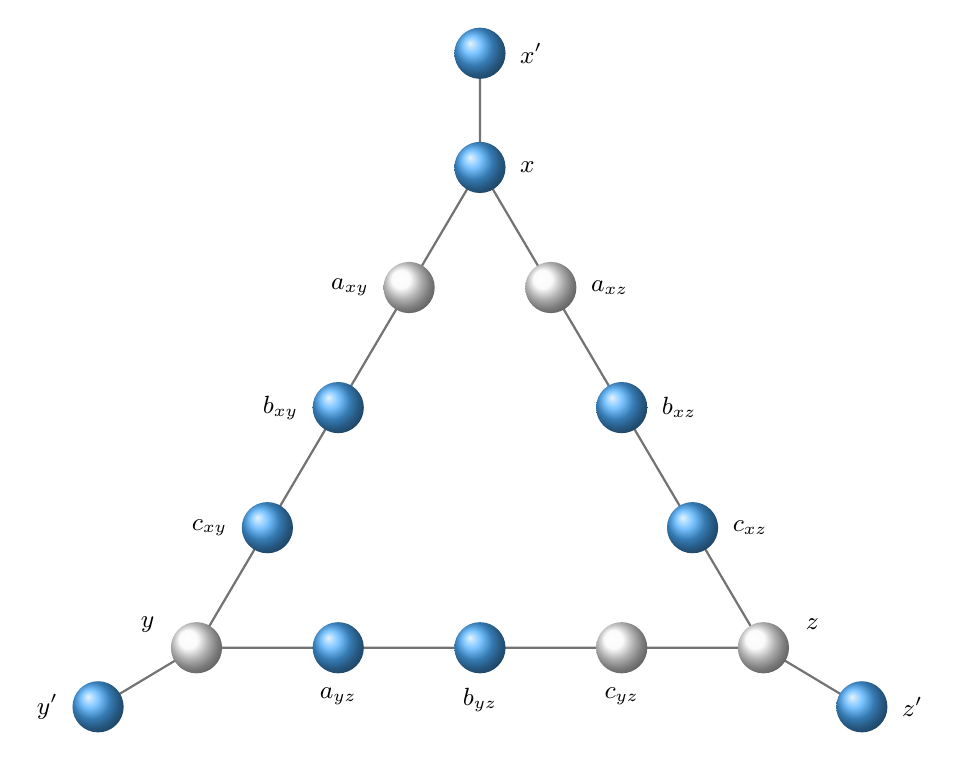
\begin{tikzpicture}[
    inS/.style={circle, minimum size=6.5mm, inner sep=0pt, shading=ball, ball color=blue!45!cyan!70},
    outS/.style={circle, minimum size=6.5mm, inner sep=0pt, shading=ball, ball color=white!95!gray},
    lab/.style={font=\small},
    e/.style={line width=0.8pt, black!55},
  ]
  \coordinate (X) at (0, 4.0);
  \coordinate (Y) at (-3.6, -2.1);
  \coordinate (Z) at (3.6, -2.1);
  % inner vertices of the three paths, at 1/4, 1/2, 3/4 from the first end
  \foreach \e/\A/\B in {xy/X/Y, yz/Y/Z, xz/X/Z} {
    \coordinate (a\e) at ($(\A)!0.25!(\B)$);
    \coordinate (b\e) at ($(\A)!0.5!(\B)$);
    \coordinate (c\e) at ($(\A)!0.75!(\B)$);
  }
  \coordinate (pX) at (0, 5.45);
  \coordinate (pY) at (-4.85, -2.85);
  \coordinate (pZ) at (4.85, -2.85);
  % edges
  \draw[e] (X) -- (Y) (Y) -- (Z) (X) -- (Z);
  \draw[e] (X) -- (pX) (Y) -- (pY) (Z) -- (pZ);
  % vertices: J({x}) = {x, x', y', z'} + all b + {c_xy, a_yz, c_xz}
  \foreach \v/\s in {X/inS, Y/outS, Z/outS, pX/inS, pY/inS, pZ/inS,
                     axy/outS, bxy/inS, cxy/inS,
                     ayz/inS, byz/inS, cyz/outS,
                     axz/outS, bxz/inS, cxz/inS} \node[\s] at (\v) {};
  % labels
  \node[lab, right=11pt] at (X) {$x$};
  \node[lab] at ($(Y)+(-0.62,0.3)$) {$y$};
  \node[lab] at ($(Z)+(0.62,0.3)$) {$z$};
  \node[lab, right=11pt] at (pX) {$x'$};
  \node[lab, left=11pt] at (pY) {$y'$};
  \node[lab, right=11pt] at (pZ) {$z'$};
  \foreach \p in {a, b, c} {
    \node[lab, left=11pt] at (\p xy) {$\p_{xy}$};
    \node[lab, below=11pt] at (\p yz) {$\p_{yz}$};
    \node[lab, right=11pt] at (\p xz) {$\p_{xz}$};
  }
\end{tikzpicture}
\end{document}
